\subsubsection{Analysis of GMRES} \label{GMRES}

The $k$th GMRES iteration minimizes the residual $r= $ over $x_0$ + $\mathcal{K}_k$, where $x_0$ is the initial iterate and $\mathcal{K}_k$ is the the $k$th Krylov subspace
$\mathcal{K_k} = \texttt{Span} \{ r_0, J \cdot r_0, . . . , J_{k-1} \cdot r_0 \}$.
Clearly, (fast) matrix-vector products play a crucial role in generating this sequence since each subsequent vector in the sequence is obtain from the previous one by multiplication by $A$.

\subsubsection{experiments}
For $N=1e^6$ particles and $\Delta_T =0.1$: variance and bias becomes lower, for decreasing GMRES-tolerance, until $\epsilon_{GMRES}= 1e-6$, then blow-up was observed.

\begin{figure}
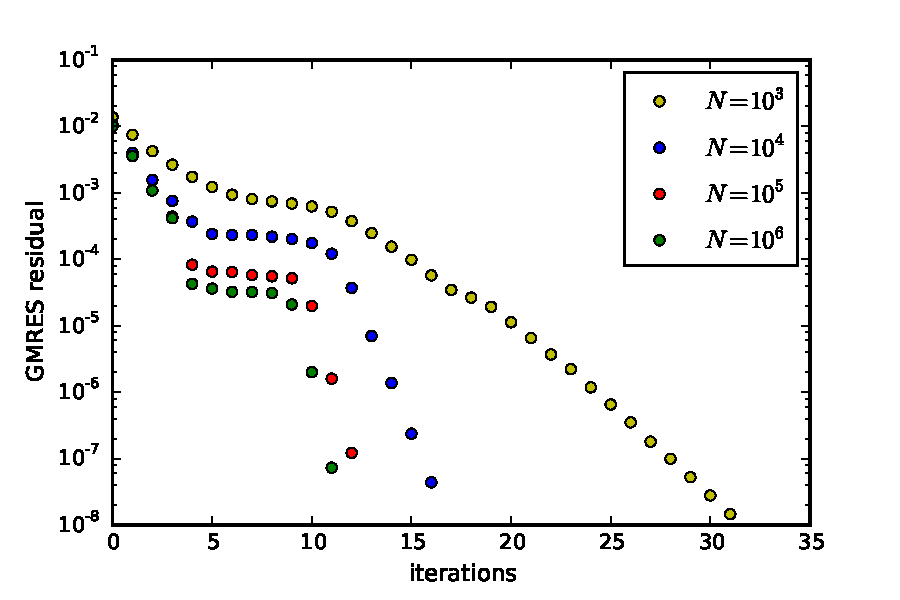
\includegraphics[width=0.5\linewidth]{../Problems/WeightedParticles/checkSystem/plots/GMRES/GMRES_N_Dt_1e-1}
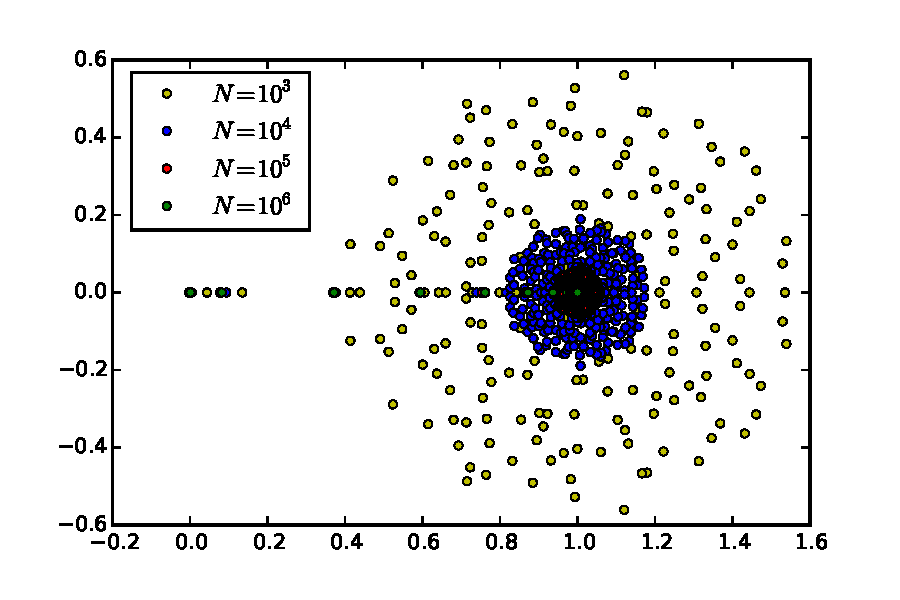
\includegraphics[width=0.5\linewidth]{../Problems/WeightedParticles/checkSystem/plots/GMRES/Spectrum_Dt_1e-1}
\caption{
\textit{Left:} The linear iterations necessary to
obtain convergence decrease as we increase the number of particles  $N$.
\textit{Right:} The linear iterations necessary to
obtain convergence depends on the spectrum of the eigenvalues of the Jacobian. The clustering radius $\rho$ decreases as we increase the number of particles  $N$.
} 
\label{fig:Spectrum_Dt_1e-1}
\end{figure}



To get a better understanding of the convergence behaviour of the GMRES-method, we refer to the following theorem.
\begin{Theorem}[Proof in \cite{broyden2004krylov} and \cite{campbell96}]
Let $ \mathbf{A} \in \mathbb{C}^{n\times n}$ and assume it has $m$ distinct eigenvalues $\lambda_i$ clustered so that for some $\rho > 0 $ and $z \in \mathcal{C}$ , $|\lambda_i - z| \leq \rho$, together with $p$ eigenvalues $\mu_i$ (outliers), each of multiplicity $m_j$ and each lying outside the cluster $|\mu_i - z| > \rho$. Let $d= \sum_{j=1}^p m_j$  so that $n= d+m$. Then, if GMRES is applied to a set of equations with such a matrix of coefficients, it follows, for $k>0$,

\begin{equation}
\| \mathbf{r}_{d+k+1} \| \leq C  \left( \frac{\rho}{|z|} \right)^k  \| \mathbf{r}_1 \| ,
\end{equation}
where $C$ is a constant not depending on $k$.
\end{Theorem}

The theorem states that GMRES may behave as if it were a two-stage process. In the first phase the terms due to the outliers are eliminated before rapid linear convergence sets in for the second phase. The rate of convergence in this second stage is determined by $\frac{\rho}{\lvert z\lvert}$, where $z$ represents the center of the cluster and  $\rho$ its radius. The closer $z$ is to the origin, the slower the expected convergence of the algoritm. If the radius of the cluster $\rho$ is small, we expect a faster convergence of the algorithm. This is observed in figure \ref{fig:Spectrum_Dt_1e-1}.


